\documentclass[11pt,letterpaper,twoside,openright]{report}
\usepackage[utf8]{inputenc}
\usepackage[english]{babel}

%preámbulo configuración de página
\usepackage[width=165mm,top=15mm,bottom=25mm,bindingoffset=20mm,includehead]{geometry}

%Preámbulo de Color de texto =================================================================
\usepackage{color}
\definecolor{gray97}{gray}{.97}
\definecolor{gray75}{gray}{.75}
\definecolor{gray45}{gray}{.45}
\definecolor{verde}{rgb}{0.0, 0.5, 0.0}

%preámbulo captions==========================================================================
\usepackage{caption}
\captionsetup{margin=40pt,format=hang,indention=-.5cm,font={footnotesize, rm},labelfont=bf,labelsep=colon}

%preámbulo encabezados=======================================================================
\usepackage{fancyhdr}
\pagestyle{fancy}
\fancyhead{}
\fancyfoot{}
\fancyhead[RO,LE]{\thepage}
\fancyhead[LO]{\nouppercase{\rightmark}}
\fancyhead[RE]{\nouppercase{\leftmark}}
\setlength{\headheight}{15pt} 


%preámbulo matemáticas=======================================================================
%\spanishdecimal{.}
\usepackage{amsmath}
\usepackage{amsfonts}
\usepackage{amssymb}
\usepackage{dsfont}
\usepackage{mathrsfs}
\newcommand{\sign}[1]{\mathrm{sign(#1)}} 
\newcommand{\refe}[1]{(\ref{#1})}
\newcommand{\rojo}[1]{{\color{red} #1}}
\newcommand{\RE}{\mathbb{R}}
\newcommand{\sig}[2]{\lceil#1\rfloor^{#2}}
\newcommand{\abs}[2]{|#1|^{#2}}
\providecommand{\norm}[1]{\lVert#1\rVert}
\usepackage{color}   
\setcounter{MaxMatrixCols}{20}
%\decimalpoint


%preámbulo sistema internacional de unidades================================================
\usepackage{siunitx}


%preámbulo referencias========================================================================
\usepackage[numbers]{natbib}
%\bibliographystyle{plainnat}
\usepackage[hidelinks, breaklinks=true, backref=page,colorlinks=true,linkcolor=blue,citecolor=magenta]{hyperref}


%preámbulo de gráficos=========================================================================
\usepackage{graphicx}
\graphicspath{{figuras/}}
\usepackage{subfigure}
\usepackage{float}

%Preámbulo tabla=============================================================================
\usepackage{multirow, array}
\usepackage{booktabs}
\usepackage{colortbl}
\definecolor{SeaGreen}{rgb}{0.13, 0.7, 0.67}
\definecolor{Peach}{rgb}{0.97, 0.51, 0.47}
\definecolor{LimeGreen}{rgb}{0.31, 0.78, 0.47}
\definecolor{bananayellow}{rgb}{1.0, 0.88, 0.21}
%preámbulo de apéndices======================================================================
\usepackage[toc,page]{appendix}
\renewcommand{\appendixpagename}{Apéndices}

%preámbulo de url============================================================================
\usepackage{url}

%preámbulo de nomenclatura==================================================================
\usepackage[intoc,spanish]{nomencl}
\makenomenclature
\usepackage{etoolbox}


%Preámbulo para código de programación=======================================================
\usepackage{listings}
\lstset{ 
	backgroundcolor=\color{white},
	rulesepcolor=\color{black},
	%
	stringstyle=\ttfamily,
	showstringspaces = false,
	basicstyle=\footnotesize\ttfamily,
	commentstyle=\color{gray45},
	keywordstyle=\bfseries,
	%
}
\renewcommand{\lstlistingname}{Listado}

%Preámbulo numeros decimales================================================================
%\spanishdecimal{.}


%preámbulo Marcadores=======================================================================
\usepackage[hidelinks, breaklinks=true, backref=page]{hyperref} 

%Redifiniendo Titulos==========================================================================
\usepackage{titlesec}
\newcommand{\bigrule}{\titlerule[0.5mm]}
\titleformat{\chapter}[display] % Se cambia el formato del capitulo
%{\bfseries\Huge} % por defecto se usarán caracteres de tamaño \Huge en negrita
{\bfseries\Huge} % por defecto se usarán caracteres de tamaño \Huge en negrita
{% contenido de la etiqueta
	\titlerule % línea horizontal
	\filright % texto alineado a la derecha
	\Large\chaptertitlename\ % "Capítulo" o "Apéndice" en tamaño \Large en lugar de \Huge
	\Large\thechapter} % número de capítulo en tamaño \Large
{0mm} % espacio mínimo entre etiqueta y cuerpo
{\filright} % texto del cuerpo alineado a la derecha
[\vspace{0.5mm} \bigrule] % después del cuerpo, dejar espacio vertical y trazar línea horizontal gruesa

%Preámbulo utilidades=========================================================================
\usepackage{pdfpages}	%Incluye hojas de de archivos PDF
\usepackage{siunitx}			%Sitema internacional de unidades
\usepackage[T1]{fontenc}	%Fuentes
\usepackage{textcomp}		%Fuentes

%preámbulo teoremas, Definiciones y Proposiciones ==============================================================================================================
\newtheorem{theorem}{Theorem}[chapter]
\newtheorem{definition}{Definition}[chapter]
\newtheorem{proposition}{Proposition}[chapter]
\newtheorem{observation}{Observation}[chapter]
\newtheorem{lemma}{Lemma}[chapter]
\newtheorem{property}{Property}[chapter]
\newtheorem{assumtion}{Assumption}[chapter]
\newtheorem{corollary}{Corollary}[chapter]

%preámbulo acronimo ===================================================
\usepackage{acronym}
\acrodef{fl}[FL]{Función de Lyapunov} \acused{fl}
\acrodef{pd}[p.d.]{positiva definida}
\acrodef{ae}[AE]{asintóticamente estable}
\acrodef{gae}[GAE]{global y asintóticamente estable}


%preámbulo de nomenclatura ==========================================
%\usepackage[intoc, spanish]{nomencl}
\makenomenclature
\nomenclature{$MCC$}{Modo de conducción continua}
%FIN DEL PREÁMBULO===================================================

%====================================================================
%====================================================================
%                    INICIO DEL DOCUMENTO
%====================================================================
%====================================================================
\begin{document}
	\chapter{Preliminaries and Theoretical framework}	
In this chapter some definitions and a brief review of necessary mathematical tools will be given in order to have a clear exposition of the problem and results. First we start with the description of systems we are working on and the Special Coordinated Basis (SCB) transformation of linear systems, required in this work to the observer design. Then we recall the well known concepts of strong observability and strong detectability giving a characterization of them in terms of the zeros and relative degree of the system. Later we state the concepts of classical and weighted homogeneity and some relevant results in functional analysis with this property, immediately we give an extension to homogeneity in the bi-limit which is part of the central axis of this work. Additionally we have to remember a few important ideas on the Lyapunov stability issue, some recent concepts such as Finite Time Stability (FTS) and Fixed Time Stability are given formally. Finally we explain how the recently introduced Bl-homogeneous differentiators are built.

Although they have already been used in the previous chapter, some important notations are as follows. For a real variable $z\in \mathbb{R}$ and a real number $p\in \mathbb{R}$ the symbol $\sig{z}{p}=\abs{z}{p}\sign{z}$ is the signed power $p$ of $z$. According to this $\sig{z}{0}=\sign{z}$, additionally $\frac{d}{dz}\sig{z}{m}=m\abs{z}{m-1}$ and $\frac{d}{dz}\abs{z}{m}=m\sig{z}{m-1}$. Note that $\sig{z}{2}=\abs{z}{2}\sign{z} \neq z^2$, and if $p$ is an odd number then $\sig{z}{p}=z^p$ and $\abs{z}{p}=z^p$ for any even integer $p$. Moreover, $\sig{z}{p}\sig{z}{q}=\abs{z}{p+q}$, $\sig{z}{p}\sig{z}{0}=\abs{z}{p}$ and $\sig{z}{0}\abs{z}{p}=\sig{z}{p}$.

\section{Description of systems and properties}
In contrast to the Single Input - Single Output (SISO) case, in the Multi Input - Multi Output (MIMO) case existing normal forms are not clearly defined in order to design Unknown Input Observers (UIO) for example the well-known classical observability canonical form by Luenberger \cite{Luenberger1967}\cite{Gupta1974} which is based on the observability indices does not take the impact of the unknown inputs into account.

\subsection{Special Coordinated Basis} 
Essentially, the so-called Special Coordinate Basis \cite{Chen2004}\cite{Sannuti1986} decomposes the multivariable linear system into coupled chains of integrators. Such that several fundamental properties of linear systems regarding controllability (stabilisability), observability (detectability), invariant zeros, decoupling zeros, infinite zero structure, effect of feedback on zero structure, squaring down, diagonal and triangular decoupling, etc. can be directly displayed in terms of the Special Coordinate Basis.

Consider a general strictly proper linear system $\Sigma$ characterized by
\begin{equation}
	\begin{split}\label{ecu: Sigma}
		\Sigma: \left\{
		\begin{array}{rl}
			\dot{x} & =Ax+Du \\
			y & = Cx
		\end{array}
		\right. \\
	\end{split}
\end{equation}

where $x\in \RE^n, u\in \RE^m$ and $y\in \RE^p$ are the state, input and output respectively. Without loss of generality, we assume that all inputs and outputs are linearly independent, i.e. both $D$ and $C$ are of full rank. Then we have the following structural or Special Coordinate Basis decomposition of $\Sigma$.

\begin{theorem}\label{theorem: SCB}
	Consider the strictly proper system $\Sigma$ characterized by \eqref{ecu: Sigma SCB}. There exist a nonsingular state transformation, $\Gamma_s \in \RE^{n\times n}$ , a nonsingular output transformation, $\Gamma_o \in \RE^{p\times p}$, and a nonsingular input transformation, $\Gamma_i \in \RE^{m\times m}$, that will reveal all the structural properties $\Sigma$. More specifically, we have
	
	\begin{equation}
		x=\Gamma_s\bar{x}, \quad y=\Gamma_o\bar{y}, \quad u=\Gamma_i\bar{u},
	\end{equation}

which transform the system into 

\begin{equation}
	\begin{split}\label{ecu: Sigma SCB}
		\Sigma_{SCB}: \left\{
		\begin{array}{rl}
			\dot{\bar{x}} & =\bar{A}\bar{x}+\bar{D}\bar{u} \\
			\bar{y} & = \bar{C}\bar{x}
		\end{array}
		\right. \\
	\end{split}
\end{equation}

with the new state variables 
\begin{equation}
	\bar{x}=
	\begin{bmatrix}
		x_a \\
		x_b \\
		x_c \\
		x_d
	\end{bmatrix}, x_a \in \mathbb{R}^{n_a}, \quad x_b \in \mathbb{R}^{n_b}, \quad x_c \in \mathbb{R}^{n_c}, \quad x_d \in \mathbb{R}^{n_d}
\end{equation}

the new output variables 
\begin{equation}
	\bar{y}=
	\begin{bmatrix}
		y_d \\
		y_b
	\end{bmatrix}, y_d \in \mathbb{R}^{p_d}, \quad y_b \in \mathbb{R}^{p_b}
\end{equation}
and the new input variables
\begin{equation}
	\bar{u}=
	\begin{bmatrix}
		u_d \\
		u_c
	\end{bmatrix}, u_d \in \mathbb{R}^{p_d}, \quad u_c \in \mathbb{R}^{m_c}
\end{equation}

Further, the stare variables $x_b$ can be decomposed as
\begin{eqnarray}
	x_b=
	\begin{bmatrix}
		x_{b,1} \\
		x_{b,2} \\
		\vdots \\
		x_{b,p_b}
	\end{bmatrix}, \quad
	y_b=
	\begin{bmatrix}
		y_{b,1} \\
		y_{b,2} \\
		\vdots \\
		y_{b,p_b}
	\end{bmatrix}, \\
	x_{b,\iota} \in \mathbb{R}^{n_{b,i}},\quad
	x_{b,\iota}=
	\begin{bmatrix}
		x_{b,\iota,1} \\
		x_{b,\iota,2} \\
		\vdots \\
		x_{b,\iota,n_{b,\iota}}
	\end{bmatrix}, \quad \iota=1,2,...,p_b,
\end{eqnarray}
with $n_{b,1} \leq n_{b,2} \leq \hdots \leq n_{b,p_b}$ and $\sum_{\iota=1}^{p_b} n_{b,\iota}=n_b$.

The state variable $x_c$ can be decomposed as
\begin{eqnarray}
	x_c=
	\begin{bmatrix}
		x_{c,1} \\
		x_{c,2} \\
		\vdots \\
		x_{c,m_c}
	\end{bmatrix}, \quad
	u_c=
	\begin{bmatrix}
		u_{c,1} \\
		u_{c,2} \\
		\vdots \\
		u_{c,m_c}
	\end{bmatrix}, \\
	x_{c,k} \in \mathbb{R}^{n_{c,k}},\quad
	x_{c,k}=
	\begin{bmatrix}
		x_{c,k,1} \\
		x_{c,k,2} \\
		\vdots \\
		x_{c,k,n_{c,k}}
	\end{bmatrix}, \quad k=1,2,...,m_c,
\end{eqnarray}
with $n_{c,1} \leq n_{c,2} \leq \hdots \leq n_{c,m_c}$ and $\sum_{k=1}^{m_c} n_{c,k}=n_c$. 

And finally, the state variable $x_d$ can be decomposed as:

\begin{eqnarray}
	x_d=
	\begin{bmatrix}
		x_{d,1} \\
		x_{d,2} \\
		\vdots \\
		x_{d,p_d}
	\end{bmatrix}, \quad
	y_d=
	\begin{bmatrix}
		y_{d,1} \\
		y_{d,2} \\
		\vdots \\
		y_{d,p_d}
	\end{bmatrix}, \quad
	u_d=
	\begin{bmatrix}
		u_{d,1} \\
		u_{d,2} \\
		\vdots \\
		u_{d,p_d}
	\end{bmatrix}, \\
	x_{d,i} \in \mathbb{R}^{n_{d_{i}}},\quad
	x_{d,i}=
	\begin{bmatrix}
		x_{d,i,1} \\
		x_{d,i,2} \\
		\vdots \\
		x_{d,i,n_{d,i}}
	\end{bmatrix}, \quad i=1,2,...,p_d,
\end{eqnarray}
with $n_{d_1} \leq n_{d_2} \leq \hdots \leq n_{d_{p_d}}$ and $\sum_{i=1}^{p_d} n_{d,i}=n_d$.

The decomposed system can be expressed in the following dynamical subsystems. First $\Sigma_a$
\begin{equation}\label{ecu: xa}
	\dot{x}_a=A_{aa}x_a + H_{ab}y_b + H_{ad}y_d
\end{equation}
$\Sigma_b$ composed by each subsystem $x_{b,\iota},\iota=1,2,...,p_b$,
\begin{equation}
	\begin{split}\label{ecu: xb}
		\dot{x}_{b,\iota,1} &= x_{b,\iota,2} + H_{bd,\iota,1}y_d, \quad y_{b,\iota}=x_{b,\iota,1}, \\
		\dot{x}_{b,\iota,j} &= x_{b,\iota,j+1} + H_{bd,\iota,j}y_d, \\
		& \vdots \quad j=1,...,n_{b,\iota}-1\\
		\dot{x}_{b,\iota,n_{b,\iota}} &= A_{bb,\iota}x_{b} + H_{bd,\iota,n_{b,\iota}}y_d, 
	\end{split}
\end{equation}

$\Sigma_c$ composed by each subsystem $x_{c,k}, k=1,2,...,m_c$
\begin{equation}
	\begin{split}\label{ecu: xc}
		\dot{x}_{c,k,1} &= x_{c,k,2} + H_{cb,k,1}y_b + H_{cd,k,1}y_d, \\
		\dot{x}_{c,k,j} &= x_{c,k,j+1} + H_{cb,k,j}y_b + H_{cd,k,j}y_d, \\
		& \vdots \quad j=1,...,n_{c,k}-1\\
		\dot{x}_{c,k,n_{c,k}} &= A_{ca,k}x_a + A_{cc,k}x_c + H_{cb,k,n_{c,k}}y_b + H_{cd,k,n_{c,k}}y_d + \omega_{c,k}, 
	\end{split}
\end{equation}
and finally, $\Sigma_d$ composed by each subsystem $x_{d,i}, i=1,2,...,p_d$
\begin{equation}
	\begin{split}\label{ecu: xd}
		\dot{x}_{d,i,1} &= x_{d,i,2} + H_{dd,i,1}y_d,  \quad y_{d,i} = x_{d,i,1} \\
		\dot{x}_{d,i,j} &= x_{c,i,j+1} + H_{dd,i,j}y_d, \\
		& \vdots \quad j=1,...,n_{c,i}-1\\
		\dot{x}_{d,i,n_{d,i}} &= A_{da,i}x_a + A_{dc,i}x_c + A_{db,i}x_b + A_{dd,i}x_d + w_{d,i}, 
	\end{split}
\end{equation}
where $A_{aa},H_{ab},H_{ad},A_{bb},H_{bd,i,j},A_{cc},A_{ca},H_{cb,k},H_{cd,k},A_{dd},A_{da},A_{dc},A_{db},H_{dd,\iota}$ are constant row vectors of appropriate dimensions. And  we consider $|w_{d,\iota}(t)|< \Delta_{\iota} \in \RE_{\geq 0}$.
\end{theorem}

\begin{figure}[H]
	\centering
	\subfigure[$x_a$ the subsystem without direct input and output.]{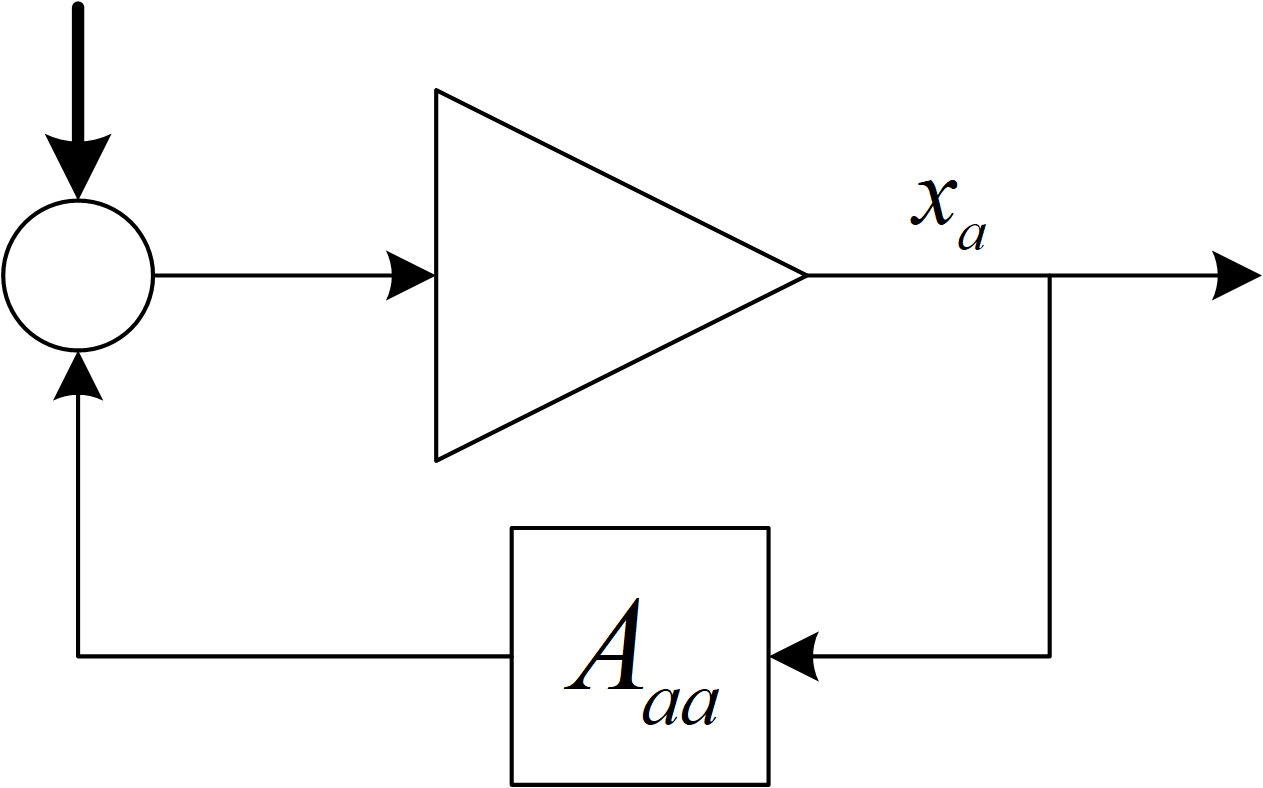
\includegraphics[scale=1]{xa.png}} \\
	\subfigure[$x_{b,\iota}$ the chain of integrators without a direct input.]{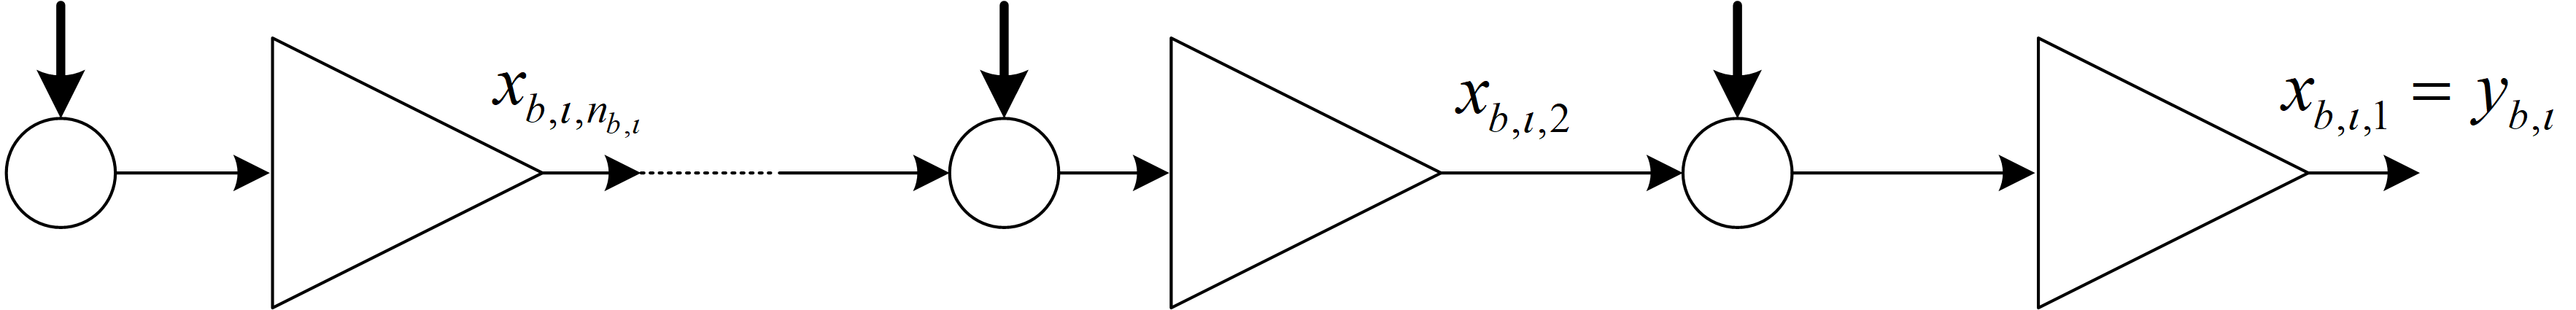
\includegraphics[scale=1]{xb.png}} \\
	\subfigure[$x_{c,k}$ the chain of integrators without a direct output.]{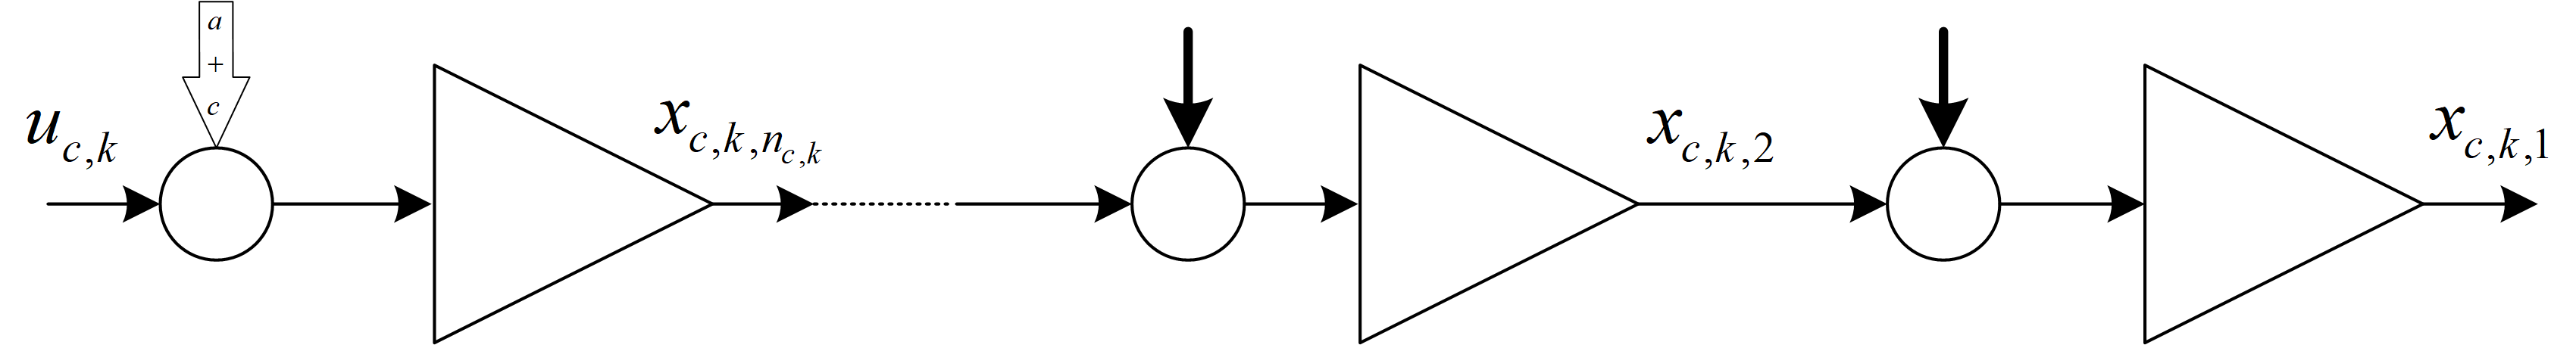
\includegraphics[scale=1]{xc.png}} \\
	\subfigure[$x_{d,i}$ the chain of integrators with direct input and output.]{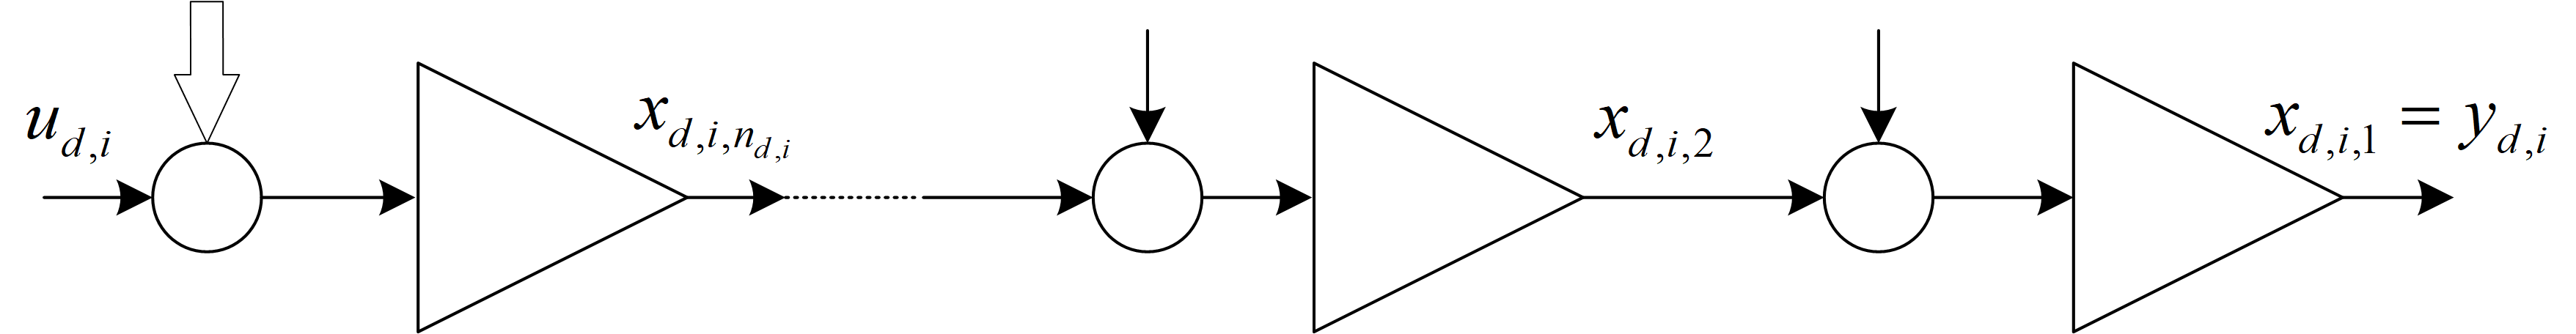
\includegraphics[scale=1]{xd.png}}
	\caption{Graphic interpretation of structural SCB decomposition of a MIMO system.}
	\label{fig: SCB}
\end{figure}

The proof of this Theorem \ref*{theorem: SCB} is given in \cite{Chen2004}. For simplicity, the system \eqref{ecu: Sigma} is considered without feedthrough (the arguments in following chapters are equally applicable with an extra steps in SCB transformation). Although the procedure for the decomposition of MIMO systems is complicated, the principal idea is the identification of chains of integrators between the system input and output variables. Three different types of chains of integrators can be identified:

\begin{enumerate}
	\item Chains that start from an input channel and end with an output. This type
	of chain gives the infinite zero structures of the given system and covers the
	subspace corresponding to $x_d$.
	\item Chains that start from an input channel but do not end with an output. This
	type of chain covers the subspace corresponding to $x_c$.
	\item Chains that do not start from an input but end with an output variable. This
	type of chain covers the subspace corresponding to $x_b$.
\end{enumerate}

These subspaces do not cover the whole state space of the given system. The remaining part forms a subspace corresponding to $x_a$, which is related to the invariant zeros of the system, i.e. the zeros dynamics. These four subsystems $x_a,x_b,x_c,x_d$ are depicted in graphical form in Figure \ref{fig: SCB}.



where the signal indicated by the double-edged arrow in $x_d$ is a linear combination of all the state variables; the signal indicated by the double-edged arrow marked with $a + c$ in $x_c$ is a linear combination of the state variables $x_a$ and $x_c$; the signals indicated by the thick vertical arrows are some linear combinations of the output variables $y_d$ and $y_b$; and the signals indicated by the thin vertical arrows are some linear combinations of the output variable $y_d$.

The subsystems have the following properties
\begin{enumerate}
	\item $\Sigma_a$ corresponds to the zeros dynamics. If $A_{aa}$ is Hurwitz then it is detectable. If not it is undetectable.
	\item Subsystem $\Sigma_b$ is not affected by the unknown input vector, and it is observable. Therefore it can be expressed in observer or observability canonical form. \eqref{ecu: xd} is expressed as the latter.
	\item Subsystem $\Sigma_c$ is affected by the unknown input, it is not strongly observable.
	\item Subsystem $\Sigma_d$ is affected by the unknown input vector, it is strongly observable, and because the number of inputs and outputs is the same $p_d$ then the subsystem is square.
\end{enumerate}

Several important properties of linear systems for this work can be displayed by the SCB, nonetheless, before that, some definitions about observability and detectability  for systems with unknown inputs have to be remembered.

\begin{definition}
	The zeros of the system \eqref{ecu: Sigma} correspond to the values $s\in \mathbb{C}$ for which the Rosenbrock's matrix 
	\begin{equation}\label{ecu: Rosenbrok}
		\begin{split}
			R(s)=
			\begin{bmatrix}
				sI-A & -D\\
				C & 0	
			\end{bmatrix}, \quad \forall s\in \mathbb{C}
		\end{split}
	\end{equation} 
	loses rank, i.e. $rank[R(s)] < n+m$.
\end{definition}

\begin{definition}
	The system \eqref{ecu: Sigma} is strongly observable if 
	\begin{equation}
		y(t)=0 \textup{ for } t>0  \quad \textup{ implies }  \quad x(t) = 0 (t > 0)
	\end{equation}
	for any input and initial state. \\
	Equivalently, the system is strongly observable if and only if it has no zeros.
\end{definition}

\begin{definition}
	The system \eqref{ecu: Sigma} is strongly detectable if 
	\begin{equation}
		y(t)=0 \textup{ for } t>0 \quad \textup{ implies }  \quad  x(t) \rightarrow 0 (t \rightarrow 0)
	\end{equation}
	for all inputs and initial states. \\
	Equivalently, the system is strongly detectable if and only if all its zeros $s$ satisfy $Re[s] < 0$.
\end{definition}
\newpage
\begin{definition}\label{def: Strong Det*}
	The system \eqref{ecu: Sigma} is strongly$^*$ detectable if 
	\begin{equation}
		y(t)\rightarrow 0 (t \rightarrow 0)  \quad  \textup{ implies }  \quad  x(t) \rightarrow 0 (t \rightarrow 0)
	\end{equation}
	for all inputs and initial states. \\
	Equivalently, the system is strongly$^*$ detectable if and only if it is strongly detectable, i.e.
	\begin{equation}\label{ecu: Fase minima}
		\begin{split}
			rank
			\begin{bmatrix}
				sI-A & -D\\
				C & 0	
			\end{bmatrix}=n+m, \quad \forall s\in \mathbb{C}
		\end{split}
	\end{equation}
	 and additionally
	\begin{equation}\label{ecu: Cond rel deg 1}
			rank(CD) = rank(D)
	\end{equation} 
\end{definition}

Consequently of these definitions strong observability implies strong detectability but it does not imply strong$^*$ detectability.

As mentioned before, all the invariant properties of the given system can be easily obtained from the structural decomposition. Then it can be now stated the next property of the system and subsystems in SCB coordinates.

\begin{property}
	The system $\Sigma_{SCB}$ in \eqref{ecu: Sigma SCB} is strong observable if and only if, $x_a$ and $x_c$ are non-existent.
\end{property}

\section{Conditions for the existence of Unknown Input Observers}
In \cite{Hautus1983}\cite{Trentelman2001} the necessary and sufficient conditions for the existence of observers for systems in which the input is not completely available for measurement were introduced, i.e. Observers with of Unknown Inputs (UIO) signals. Such conditions are described in terms of the properties before mentioned related to the structure of the system. 

\begin{theorem}
Under the assumption that the unknown input $\omega(t)$ is a completely arbitrary signal, e.g. it may be unbounded. The system $\Sigma$ in \eqref{ecu: Sigma} has a Unknown Input Observer if and only if it is Strong Detectable$^*$, i.e.

\end{theorem}

This, in Definition \ref{def: Strong Det*} is equivalent to have minimum phase condition, since the rank of the Rosenbrock matrix has to be equal to $n + m, \forall s\in \mathbb{C}$ or the absence of invariant zeros. And, from \eqref{ecu: Cond rel deg 1} a relative degree one condition. Based on the definition we can emphasize:

\begin{observation}
	Strong detectability or even strong observability is not sufficient for the existence of an Unknown Input Observer.
\end{observation}

Since the conditions of minimum phase and relative degree one are necessary and sufficient, it is impossible to overcome them without imposing another restrictions to the problem formulation. Hereafter the following is assumed

\begin{assumtion}
	The unknown input $\omega(t)$ is uniformly bounded, i.e. there exist some $\Delta \in \RE_{\geq 0}$ such that $\norm{\omega(t)}<\Delta$.
\end{assumtion}

\section{Homogeneity and Bl-homogeneity}
Homogeneity is the property whereby objects such as functions or vector fields scale in a consistent fashion with respect to a scaling operation called a dilation \cite{Bernuau2014}, which is essentially an action of the multiplicative group of positive real numbers on the state space \cite{Bhat2005}. Homogeneity with respect to the standard dilation is one of the two axioms for linearity, the other being additivity. Many familiar properties of linear systems follow, in fact, from homogeneity alone. The first step of homogeneity consists in homogeneous polynomials. The Euler’s homogeneous function theorem was the first result linking homogeneity with analysis. And in control theory, homogeneity appeared with Lasalle and Hahn in the 40’s. 

\begin{definition}
	Let $n$ and $m$ be two positive integers. A mapping $f: \RE^n \rightarrow \RE^m$ is said to be homogeneous (in the classical sense) with degree $l \in \RE$ if and only if $\forall \epsilon>0: \quad f(\epsilon x) = \epsilon^lf(x)$.
\end{definition}

The main issue with the classical homogeneity was its very restrictive field of use. Hence, a generalization of the classical homogeneity was proposed by V.I. Zubov in 50s and developed by H. Hermes in the 90’s using different weights, leading to weighted homogeneity. Nowadays, this is the most popular definition of homogeneity \cite{Bernuau2014}.

\begin{definition}
	Fix a set of coordinates $(x_1,...,x_n)\in \RE^n$. Let $\epsilon>0$ all real numbers and $r=(r_1,...,r_n)$ be a n-upled of positive real numbers. The dilation operator is defined as $\Delta_{\epsilon}^{r}x = \left[ \epsilon^{r_1}x_1,...,\epsilon^{r_n}x_n \right]^T$, where the numbers $r_i$ are the weights of the coordinates. The map also can be written as $\Delta_{\epsilon}^{r}x = diag(\epsilon^{r_1},...,\epsilon^{r_n})x$, where $\Delta_{\epsilon}^{r}$ is the dilation matrix and $x$ the vector of coordinates.
\end{definition}

\begin{definition}
	It is said that
	\begin{itemize} 
		\item A function $V: \RE^n \rightarrow \RE$ is $r$-homogeneous of degree $l$ or $(r,l)$-homogeneous for short, if the equality $V(\Delta_{\epsilon}^{r}x) = \epsilon^lV(x), \forall x\in \RE^n  \textbackslash \{0 \}, \forall \epsilon >0$ holds.
		\item A vector field $f: \RE^n \rightarrow \RE^n$ is $r$-homogeneous of degree $l$, if the equality $f(\Delta_{\epsilon}^{r}x) = \epsilon^l \Delta_{\epsilon}^{r} f(x), \forall x\in \RE^n  \textbackslash \{0 \}, \forall \epsilon >0$ holds.
		\item A vector-set field $F: \RE^n \rightrightarrows\RE^n$, $F(x), \subset \RE^n$ is $r$-homogeneous of degree $l$, if the equality $F(\Delta_{\epsilon}^{r}x) = \epsilon^l \Delta_{\epsilon}^{r} F(x), \forall x\in \RE^n  \textbackslash \{0 \}, \forall \epsilon >0$ holds.
		\item A system $\dot{x} = f(x)$ is homogeneous if and only if $f$ is so.
	\end{itemize}
\end{definition}

An extension to this concept has is the homogeneity in the bi-limit or bl-homogeneity for short.

\begin{definition}
	A function $\varphi: \RE^n \rightarrow \RE$ is said to be homogeneous in the $0$-limit with associated triple $(r_0,l_0,\varphi_0)$, if it is approximated near $x=0$ by the $(r_0,l_0)$-homogeneous function $\varphi_0$. It is said to be homogeneous in the $\infty$-limit with associated triple $(r_{\infty},l_{\infty},\varphi_{\infty})$, if it is approximated near $x=\infty$ by the $(r_{\infty},l_{\infty})$-homogeneous function $\varphi_{\infty}$. Similar definitions apply for vector fields and set-valued vector fields.
	
	Consequently, a function $\varphi: \RE^n \rightarrow \RE$ (or a vector field or set-valued vector field) is said to be homogeneous in the bi-limit if it is homogeneous in the $0$-limit and homogeneous in the $\infty$-limit.
\end{definition}

There are several results related to the homogeneity of functions, which are going to be useful for the stability analysis in the following chapters. Here we recall some of them. Fisrstly, let us mention that the regularity of a homogeneous mapping $f$ is related to its degree:

\begin{theorem}\label{theo: Regularity}
	Suppose $f: \RE^n \rightarrow \RE$ is continuous on $\RE^n \textbackslash \{0 \}$ and homogeneous of degree $l$. Then
	\begin{itemize}
		\item If $l<0$, the $f$ is continuous on $\RE^n$ if and only if $V\equiv 0$.
		\item If $l=0$, the $f$ is continuous on $\RE^n$ if and only if $V\equiv V(0)$.
		\item If $l>0$, the $f$ is continuous on $\RE^n$.
	\end{itemize}
\end{theorem}
The proof of this Theorem \ref{theo: Regularity} is given in \cite{Bhat2005}. 

The following lemma asserts that sign-definite, homogeneous functions are radially unbounded.

\begin{lemma}
	Suppose $V: \RE^n \rightarrow \RE$ is continuous and homogeneous, then
	\begin{itemize}
		\item If $V$ is sign definite, then $V$ is radially unbounded.
		\item If $n>1$ and $V$ is proper, then $V$ is sign definite.
	\end{itemize}
\end{lemma}

This property is useful in the task of Lyapunov functions construction. Another useful result, but in bl-homogeneous functions, which going to be used in the proof of main result is as follows.

\begin{lemma}
	Let $\gamma: \RE^n \rightarrow \RE$ and  $\eta: \RE^n \rightarrow \RE_{\leq 0}$ be two upper semicontinuous (u.s.c.) single-valued bl-homogeneous functions, with the same weights $r_0$ and $r_1$, degrees $m_0$ and $m_{\infty}$, and approximating functions $\eta_{0},\eta_{\infty}$ and $\gamma_0,\gamma_{\infty}$ which are u.s.c. Suppose that $\forall x\in\RE^n$, $\gamma(x)\leq 0$, $\gamma_0(x)\leq 0$, $\gamma_{\infty}(x)\leq 0$. If $\gamma(x)=0 \wedge x\neq 0 \Rightarrow \eta(x)<0$, $\gamma_{\iota}(x)=0 \wedge x\neq 0 \Rightarrow \eta_{\iota}(x)<0$ for $\iota \in \{0,\infty\}$, then there are constants $\lambda^*\in\RE$, $c_0>0,c_{\infty}>0$ such that for all $\lambda \geq max\{\lambda_0,\lambda_{\infty}\}, \lambda_0 \geq \lambda^*$, $\lambda_{\infty}>\lambda^*$ and for all $x\in \RE^n \textbackslash \{0 \}$,
	\begin{equation}
		\begin{split}
		\eta(x)+\lambda\gamma(x) \leq -c_0\norm{x}_{r_0,p}^{m_0} - c_{\infty}\norm{x}_{r_{\infty},p}^{m_{\infty}}, \\
		\eta_{\iota}(x)+\lambda\gamma_{\iota}(x) \leq -c_{\iota}\norm{x}_{r_{\iota},p}^{m_{\iota}}, \quad \iota \in \{0,\infty\}
		\end{split}
	\end{equation}
\end{lemma}


\subsection{Stability of homogeneous systems}
There are some crucial stability results that appear in the literature for the special case of systems that are homogeneous with respect to dilations of the form  $\Delta_{\epsilon}^{r}x$. But before presenting them, we formalize the concepts of stability, and the classical results in Lyapunov stability will be remembered.

\begin{definition}
	Consider the autonomous system 
	\begin{equation}\label{ecu: sys Lyap}
		\dot{x}=f(x)
	\end{equation}
	whit $f: \RE^n \rightarrow \RE^n$. Then \\
	The equilibrium point $x=0$ of \eqref{ecu: sys Lyap} is 
	\begin{itemize}
		\item Stable if, for each $\epsilon>0$, there is $\delta=\delta(\epsilon)>$0 such that 
		\begin{equation}
			\norm{x(0)} < \delta \Rightarrow \norm{x(t)}<\epsilon, \forall t\geq 0
		\end{equation}
		\item Unstable if it is not stable.
		\item Asymptotically stable if it is stable  and $\delta$ can be chosen such that
		\begin{equation}
			\norm{x(0)} < \delta \Rightarrow \lim_{t\to \infty} x(t)=0
		\end{equation}
	\end{itemize}
\end{definition}

The well known Lyapunov's stability theorem is as follows, taken from \cite{Khalil2003}

\begin{theorem}
	Let $x=0$ be an equilibrium point for \eqref{ecu: sys Lyap} and $D\subset \RE^n$ be a domain containing $x=0$. Let $V: D\rightarrow \RE$ be a continuously differentiable function such that
	\begin{equation}
		\begin{split}
		V(0) = 0 \quad and \quad V(x) &> 0 \quad in \quad D \textbackslash \{0 \} \\
		\dot{V}(x) &\leq 0 \quad in \quad D
		\end{split}
	\end{equation}
	Then, $x=0$ is stable. Moreover, if 
	\begin{equation}
		\dot{V}(x) < 0 \quad in \quad D \textbackslash \{0 \}
	\end{equation}
	then, $x=0$ is asymptotically stable.
\end{theorem}

This is local result, which can be extended to globally stability as shown in the next theorem

\begin{theorem}
		Let $x=0$ be an equilibrium point for \eqref{ecu: sys Lyap}. Let $V: \RE^n \rightarrow \RE^n$ be a continuously differentiable function such that
	\begin{equation}
			V(0) = 0 \quad and \quad V(x) > 0 \quad \forall x \neq 0 \\
	\end{equation}
	$V$ is radially unbounded, i.e.
	\begin{equation}
		\norm{x} \rightarrow \infty \Rightarrow V(x) \rightarrow \infty
	\end{equation}
	and
	\begin{equation}
		\dot{V}(x) < 0 \quad \forall x\neq 0
	\end{equation}
	then, $x=0$ is globally asymptotically stable.
\end{theorem} 

Before giving some results related to homogeneous systems, we will recall a few definitions about stability in some stronger sense. 

\begin{definition}
	\cite{Bhat2005} The system \eqref{ecu: sys Lyap} is said to be finite-time stable (FTS) at the origin (on an open neighborhood $\mathcal{V} \subset \RE^n$ of the origin) if:
	\begin{itemize}
		\item There exists a funtion $\delta\in \mathcal{K}$ such that for all $x_0\in \mathcal{V}$ we have $\norm{(x_0)}\leq \delta(\norm{x_0})$ for all $t\geq 0$.
		\item There exists a function $T:\mathcal{V}\textbackslash \{0 \} \rightarrow \RE_{+}$ such that for all $x_0\in \mathcal{V}\textbackslash \{0 \}$, $x(x_0)$ is defined, unique, nonzero on $[0,T(x_0))$ and $\lim_{t\rightarrow T(x0)}x(x_0) = 0$. $T:\RE^n \rightarrow \RE_{+} \cup \{0\}$ is the settling-time function.
	\end{itemize}
	If $\mathcal{V}=\RE^n$, the the system is called globally FTS.
	
	For differential inclusions (DI) the notion has been defined to deals with all solutions originated from a given initial condition. Details can be seen in the reference.
\end{definition}

Finally, the fixed-time (FxT) stability is a particular case of the FTS property.

\begin{definition}
	The system \eqref{ecu: sys Lyap} is said to be FxT stable at the origin if it is globally FTS and the settling-time function $T$ is bounded, i.e. $\exists \bar{T}>0$ such that $T(x)<\bar{T}$ for all $x\in \RE^n$.
\end{definition}

\subsection{Homogeneous Lyapunov functions}
Now we are completely ready to set down the some principal implications about stability for homogeneous and bl-homogeneous systems, these are important because the observer construction in the next chapter keeps this properties, which will be useful in the mathematical proofs of stability and convergence. 

\begin{theorem}
	Let \eqref{ecu: sys Lyap} be a homogeneous system, if the origin a locally stable equilibrium point, then the origin os globally asymptotically stable.
\end{theorem}

It is well known that an Asymptotically Stable linear system possesses a strict Lyapunov function which is a quadratic form. It turns out that any homogeneous Asymptotically Stable system admits a homogeneous strict Lyapunov function, not necessarily quadratic. The following theorem formalize the existence of a Lyapunov function for a homogeneous system

\begin{theorem}\label{theo: Hom V}
	\cite{BacciottiAndRosier2005} Let $f$ a continuous vector field on $\RE^n$ such that the origin is a locally asymptotically stable equilibrium point. Assume that $f$ is $r$-homogeneous of degree $m$ with $r \in (0,+\infty)^n$. Then, for any $k\in \mathbb{N}$ and any $p > k\cdot max_i\{r_i\}$, there exists a strict Lyapunov function $V$ for the system \eqref{ecu: sys Lyap}, which is $r$-homogeneous of degree $p$ and of class $\mathcal{C}^k$. As a direct  consequence, the time derivative $V=\langle \nabla V,f \rangle$ is $r$-homogeneous of degree $m+p$.
\end{theorem} 

The following corollary shows that the rate convergence of trajectories for homogeneous asymptotically stable system is completely characterized by the degree of the field.

\begin{corollary}
	Let $f$ be as in \ref{theo: Hom V}, and let $\norm{\cdot}_{r,p}$ be any $r$-homogeneous norm.
	\begin{itemize}
		\item If $k<0$, then the origin is finite-time stable.
	\end{itemize}
\end{corollary}

There are some important points 
\begin{observation}\label{obs: Sys Homogeneous}
	In homogeneous systems we have that
\begin{itemize}
	\item Finite Time Stability (FTS) is equivalent to an infinite eigenvalue assignation for the closed-loop system at the origin, therefore the right-hand side of the ordinary differential equation cannot be locally Lipschitz at the origin.
	\item There exists the settling time function $T(x_0)$ that determines the time for a solution to reach the equilibrium, this function depends on the initial condition of a solution. In general this function $T$ can grow unboundedly (possibly more than linearly).
\end{itemize}
\end{observation}

The main issue with $T$ is its continuity at the origin. For continuous systems, the continuity of $T$ at $0$ is equivalent to the continuity of $T$ everywhere. The bi-limit homogeneity application allows us to have a globally bounded $T$, which means that in practice one gets a FxT convergence to the origin for all initial conditions.

A recently application of bl-homogeneity to the observation problem is in the differentiators development with correction terms having the property of being homogeneous in the bi-limit, therefore, under some assumptions of uniform bounding the observer is able to estimate exactly in FxT the true derivatives of a signal $f$. In fact, these results are closely linked to this work. More details will be given immediately.

\newpage
\section{Arbitrary Order Fixed-Time Differentiators}
\cite{Moreno2021} Given a signal $f(t)$ defined on $[0,\infty)$, the objective is to estimate some of its time derivatives. $f(t)$ is composed of a base signal $f_0$ n-times differentiable, and a uniformly bounded noise $v(t)$, i.e.$f(t)=f_0(t)+v(t)$ and $|f_0^{(n)}(t)|\leq \Delta$ with $\Delta \geq 0$.

Defining the variables $\varsigma_1=f_0(t), \varsigma_2=\dot{f}_0(t), .... ,\varsigma_n=f_0^{(n-1)}(t)$, where $f_0^{(i)}(t)=\frac{d^i}{dt^i}f_0(t)$. A state representation of $f_0$ is
\begin{equation}
	\begin{split}
		\dot{\varsigma}_i &= \varsigma_{i+1} \qquad i=1,...,n-1 \\
		\dot{\varsigma}_n &= f_0^{(n)}(t)
	\end{split}
\end{equation}

In order to estimate the derivatives $f_0^{(i)}(t)$ for $i=1,...,n-1$ we have the following nonlinear family of differentiators
\begin{equation}\label{ecu: dif Mor}
	\begin{split}
	\dot{x}_i &= -k_i\phi_i(x_1-y)+x_{i+1}, \qquad i=1,...,n-1 \\
	\dot{x}_n &= -k_n\phi_n(x_1-y)
	\end{split}
\end{equation}
where the nonlinear output injection terms, given by
\begin{equation}
	\phi_i(z) = \varphi_i \circ ...\varphi_2 \circ \varphi_1(z)
\end{equation} 
are the composition of the monotonic growing functions
\begin{equation}\label{ecu: varphi}
	\varphi_i(s) = \kappa_i \lceil s \rfloor^{\frac{r_{0,i+1}}{r_{0,i}}} + \theta_i \lceil s \rfloor^{\frac{r_{\infty,i+1}}{r_{\infty,i}}} 
\end{equation}
with powers selected as $r_{0,n}=r_{\infty,n}=1$, and for $i=1,...,n+1$
\begin{equation}
	\begin{split}
	r_{0,i} = r_{0,i+1}-d_0 = 1-(n-i)d_0 \\
	r_{\infty,i} = r_{\infty,i+1}-d_\infty = 1-(n-i)d_\infty
	\end{split}
\end{equation}
which are completely defined by two parameters $-1 \leq d_0 \leq d_\infty < \frac{1}{n-1}$. With this selection the first term in \eqref{ecu: varphi} is dominating for small values of $s$, while the second one is dominating for large values of $s$.

Differentiator (\ref{ecu: dif Mor}) is not homogeneous, but it is homogeneous in the bi-limit, that is, near to the origin it is approximated by a homogeneous system of degree $d_0$ and far from the origin it is approximated by a homogeneous system of degree $d_\infty$. Although the scaling properties of the homogeneous systems are lost, the design of bl-homogeneous differentiators is more flexible, since the properties near the origin and far from it can be assigned independently.

If we select $d_0 = d_1 = d$ the differentiator \eqref{ecu: dif Mor} becomes homogeneous. And making $d = 0$ it is obtained the High-Gain differentiator, for $d = -1$ Levant’s robust and exact differentiator is recovered and for other values of $d$ the family of continuous differentiators in \cite{CruzZavala2016}\cite{Sanchez2018}\cite{CruzZavala2019}\cite{Jbara2021} is attained. For polynomial signals note that if $d < 0$ (resp. $d = 0$) the estimation converges in finite-time (resp. exponentially). For $d > 0$ the convergence is asymptotic, but it attains any neighborhood of zero in a time which is uniform in the initial conditions.

A particular case of interest for the differentiator is a property that is only achieved when $d0 = -1$. In that case $\phi_n$ is discontinuous and it induces a Higher-Order Sliding-Mode at the origin, allowing the estimation to converge (in the absence of noise) exactly, robustly and in finite-time to the real values of the signal derivatives when the $n$-th derivative of the signal is bounded by a non zero constant $\Delta \in \RE_{\geq 0}$, i.e. $|f_0^{(n)}(t)|\leq \Delta$. For all other values of $d_0 > -1$, the convergence is only achieved if $\Delta=0$.

As we mentioned in \ref{obs: Sys Homogeneous}, one of the disadvantages in homogeneous (including Levant’s exact) differentiators with $d_0 < 0$, is that the convergence time, although finite, grows unboundedly (and faster than linearly) with the size of the initial estimation error. One of the nice features of the bl-homogeneous design in general and of the proposed differentiator \eqref{ecu: dif Mor} in particular, is that assigning a positive homogeneity degree to the $\infty$-limit approximation $d_{\infty} > 0$ and a negative homogeneity degree to the $0$-limit approximation $d_0 < 0$, it is possible to counteract this effect: Convergence of the estimation will be achieved in Fixed-Time \cite{Moreno2021}.

The main result of this differentiators \eqref{ecu: dif Mor} can be expressed formally as follows. In the absence of noise, it is able to estimate asymptotically the first $n-1$ derivatives of the signal $f_0(t)$. Let $\mathscr{F}^{n}_{0} \triangleq \left\lbrace f^{(n)}(t) \equiv 0 \right\rbrace$ represent the class of polynomial signals and $\mathscr{F}^{n}_{\Delta} \triangleq \left\lbrace \left| f^{(n)}(t)\right| \leq \Delta \right\rbrace$ corresponds to the class of $n$-Lipschitz signals.

\begin{assumtion}\label{asump: blh differentiator}
	$f(t)=f_0(t)+\nu(t)$, with $f_0(t)$ $n-$times differentiable, $|f^{(n)}(t)|\leq \Delta$, and $\nu(t)$ a uniformly bounded measurable signal.
\end{assumtion}
Then it is possible to have the following statement

\begin{theorem}\label{theo: est diff blh}
	\cite{Moreno2021} Let the function $f(t)=f_0(t)$ be such that Assumption \ref{asump: blh differentiator} is fulfilled. Select $-1 \leq d_0 \leq d_\infty < \frac{1}{n-1}$ and choose arbitrary positive (internal) gains $\kappa_i>0$ and $\theta_i>0$, for $i=1,...,n$. Suppose that either $\Delta=0$ or $d_0=-1$. Under this conditions, and in the absence of noise ($\nu(t) \equiv 0$) there exist appropriate gains $k_i>0$, for $i=1,...,n$, such that the solutions bl-homogeneous differentiator \eqref{ecu: dif Mor} converge globally and asymptotically to the derivatives of signal, i.e. $x_i(t) \rightarrow f_0^{(i-1)}(t)$ as $t \rightarrow \infty$. In particular, they converge in Fixed-Time, i.e. $\exists \bar{T}>0$ such that for any $x_i(0) \in \mathbb{R}^n$, $x_i(t) \equiv f_0^{(i-1)}(t)$ for $t \geq \bar{T}$ for $i=1,...,n$ if either
	\begin{eqnarray*}
		&(a)& \quad -1 < d_0 < 0 < d_\infty < \frac{1}{n-1} \quad and \quad f(t)\in \mathscr{F}^{n}_{0},  \quad or \\
		&(b)& \quad -1 = d_0 < 0 < d_\infty < \frac{1}{n-1} \quad and \quad f(t)\in \mathscr{F}^{n}_{\Delta}.
	\end{eqnarray*}
\end{theorem}

The proof of this Theorem \ref{theo: est diff blh}, which is of essential importance in this work is given in the the Apendix A and detailed in \cite{Moreno2021}.

This differentiator can be seen as an observer for a special type of SISO systems, composed by a chain of $n$ integrators and with a unknown input. The idea of this work is generalizing this observer to a family of MIMO-LTI systems by decomposing the original system in a set of subsystems and designing a bl-homogeneous observer composed by a set of sub-observers with unknown inputs. And proof that the convergence is achieved exactly and in fixed time by appropriately selecting the set of gains in the observer. 

With the necessary theory of homogeneous and bl-homogeneous systems given in this chapter, we are ready to present the main contribution of this work in Chapter 3.



%Observer
%It is important to note that observer (17)-(19) is not a simple use of a HOSM differentiator, replacing the ideal derivatives in observer (16), but it is an observer, with discontinuous injection terms.





	%====================================================================
	%                          Bibliografia
	%====================================================================
	\bibliographystyle{ieeetr} 
	\bibliography{Citas}
\end{document}